% This is an example of how to use the "npsthesis" document style for theses
% Modified for personal use by Fabrice Ardhuin, 2001/03/10
%
%  TO DO : add http://upload.wikimedia.org/wikipedia/commons/d/db/Munk_ICCE_1950_Fig1.svg  in ch1 

\documentclass[a4paper]{book}  % psfig for Encapsulated PostScript
%\usepackage{fullpage}
\addtolength{\oddsidemargin}{-0.4in} \addtolength{\evensidemargin}{-1.1in}
\addtolength{\textwidth}{1.5in} \addtolength{\topmargin}{-0.5in}
\addtolength{\textheight}{1.4in}
\usepackage[pdftex]{graphicx}
\usepackage{amsmath}
\usepackage{bm}
\pdfcompresslevel9
\usepackage[american]{babel}
% %\usepackage{upmath}
\usepackage[latin1]{inputenc}
%\usepackage[pdflatex]{graphics}
\usepackage{makeidx}
\usepackage{hyperref}
\usepackage{float}
\usepackage[section]{placeins}
 \usepackage{xcolor}
\hypersetup{
    colorlinks,
    linkcolor={red!50!black},
    citecolor={blue!50!black},
    urlcolor={blue!80!black}
}

%\usepackage[pdftex,plainpages=false]{hyperref}
\usepackage{natbib}
\setlength{\bibsep}{0em}

%\degree{Doctor of Philosophy In Oceanography}

% these macros save typing:
\newcommand{\beq}{\begin{equation}}
\newcommand{\beqa}{\begin{eqnarray}}
\newcommand{\eeq}{\end{equation}}
\newcommand{\eeqa}{\end{eqnarray}}
%
%\newcommand\p3{Part 3}
%\newcommand\p2{Part 2}
%\newcommand\p1{Part 1}

%   don't have right font for script R, so use:
\renewcommand{\Re}{{\cal R}}
\providecommand\boldsymbol[1]{\mbox{\boldmath $#1$}}
\providecommand\bnabla{\boldsymbol{\nabla}}
\providecommand\bcdot{\boldsymbol{\cdot}}
\providecommand\upi{\pi}
\newcommand\biS{\mathbf{S}}
\newcommand\cb{\mathbf{c}}
\newcommand\Cb{\mathbf{C}}
\newcommand\Mb{\mathbf{M}} 
\newcommand\dr{\mathrm{d}}
\newcommand\er{\mathrm{e}}
\newcommand\etb{\mathbf{\eta}}
\newcommand\ir{\mathrm{i}}
\newcommand\hu{\widehat{u}}
\newcommand\hv{\widehat{v}}
\newcommand\hw{\widehat{w}}
\newcommand\uL{\overline{u}^L}
\newcommand\wL{\overline{w}^L}
\newcommand\Eb{\mathbf{E}}
\newcommand\Sb{\mathbf{S}}
\newcommand\Ub{\mathbf{U}}
\newcommand\ub{\mathbf{u}}
\newcommand\xb{\mathbf{x}}
\newcommand\Kb{\mathbf{K}}
\newcommand\kb{\mathbf{k}}
\newcommand\kpb{\mathbf{k^{\prime}}}
\newcommand\lb{\mathbf{l}}
\newcommand\zerob{\mathbf{0}}
\newcommand\Deltab{\mathbf{\Delta}}
\newcommand\etal{\mbox{\textit{et al.}}}
\newcommand\etc{etc.\ }
\newcommand\eg{e.g.\ }
\newcommand\Real{\mathrm{Real}}
\newcommand\Frou{\mbox{\textit{Fr}}}  % Froude number
\newcommand\ttz{\ensuremath{\rightarrow 0}}
\newcommand\Ur{\mbox{\textit{Ur}}}  % Ursell number
\newcommand\Vb{\mathbf{V}}
\newcommand\zb{\overline{\zeta}}  
\newcommand\zL{\overline{\zeta}^L}

\def\sfbsL{\mathsfbi{L}}
\def\sfbsV{\mathsfbi{V}}
\def\sfbsD{\mathsfbi{D}}
\def\d{.}    % decimal mark

\newcommand{\boxedeqn}[1]{%
  \[\fbox{%
      \addtolength{\linewidth}{-2\fboxsep}%
      \addtolength{\linewidth}{-2\fboxrule}%
      \begin{minipage}{\linewidth}%
      \begin{equation}#1\end{equation}%
      \end{minipage}%
    }\]%
}


\begin{document}
\title{{\Huge Ocean waves in geosciences }
{\Large \\  parts 1 and 2: general wave topics from deep to shallow water}
 \vspace{0.1cm}\\
   \centerline{\includegraphics[width=\textwidth]{FIGURES/couvfig_en.pdf}}}
%%%%%%%%%%%%% figure
%\begin{figure}
%\centerline{\includegraphics[width=0.7\textwidth]{couv_cours.eps}}
%\vspace{3.64in}
%\end{figure}
%%%%%%%%%%%%% end of figure
\author{Fabrice Ardhuin, \\
Laboratoire d'Oc{\'e}anographie Physique et Spatiale, Brest,
France \\
doi:  10.13140/RG.2.2.16019.78888/11 \\
\vspace{0.1cm}\\
} \maketitle
 \cleardoublepage
\pagenumbering{roman}

\setcounter{page}{3}

\tableofcontents
\cleardoublepage


%\mainmatter
\setcounter{chapter}{0}

\pagenumbering{arabic}
\chapter*{Foreword}\label{foreword}
There are countless scholarly articles and books about ocean waves, with many different points of view, going from 
mathematical treatises to naval architecture. Among these we can single out the excellent textbooks by 
\cite{Kinsman1965}, \cite{Dean&Dalrymple1991},  
and \cite{Holthuijsen2007}, the engineering manual from the \cite{USACE2002}, and many excellent scientific 
monographs by \cite{Phillips1977}, \cite{Dingemans1997a}, \cite{Young1999}, \cite{Lavrenov2003}, \cite{Janssen2004}, \cite{Lannes2013} ...  

So why another one? 

First of all, scientific developments never stop, making these previous works not obsolete but less up to date 
and complete. This will happen with the present book, even if I am trying to update it on a regular basis. The parts 1 and 2 
and the associated teaching material (jupyter notebooks ...)  is designed to be at the level of Master students in oceanography. 

Second, and more important, all these books, except possibly the jewel by \cite{Phillips1977} have a rather narrow 
scope, and do not cover aspects for which no recent monograph exist. I particularly think about microseisms, infragravity waves or 
measurement techniques including satellite remote sensing. Some of these topics are only treated in part 3.

Working with coastal engineers, geomorphologists and seismologists, has motivated me to bring to 
the forefront those results that are often obscure or very hard to follow. My point of view is that 
ocean waves play a very particular role in the Earth System, both as an important element of air-sea or land-ocean exchanges, and also as a deforming mirror that 
modifies our measurements of ocean properties using remote sensing and even in situ techniques. As a result, much insight and cross-fertilization 
can come from the integration of many geoscientifc fields, from 
microseisms to remote sensing, as well as applied disciplines such as marine meteorology or coastal and ocean engineering.
At the very least, these different disciplines are providing new data, tools, and different points of view that complement each other 
in constraining  our physical understanding of wave processes, and the parameterizations used in numerical models or remote sensing algorithms. 

On these topics, I have tried to be clear without compromising the 
accuracy of the results, but this is a very difficult balance. If you find it unclear, do not hesitate to contact me
and I will try again to clarify in the next revision. I shall finish with a final warning:  my selection of topics is clearly biased to my own tastes and 
interests, which are clearly favouring geosciences versus engineering. It does not mean that the topics ignored here are not important. 
For example, a good discussion of 
extreme waves and sea state analysis would be much more useful for all engineers 
than our development on three-dimensional wave-current interactions. For this you may go to section 4.3 of \cite{Holthuijsen2007} or, with more details, to \cite{Boccotti2000}.
I hope that the present book will be a good combination 
of useful and interesting topics. \\

\vspace{0.5cm}
The document is organized in three parts, one relevant to waves in deep water, another providing additional 
information on coastal and shallow water aspects, and a third part that goes into some details that are probably not relevant for 
most readers. This book is designed to make it easier to read in electronic form, including hypertext links within the document 
and towards outside sources, such as the cited references. It is designed as a teaching material for the wave-related Master courses 
at University of Brest and ENSTA-Paris Tech. Because the present document is trying to follow the latest 
advances in research -- and my imperfect understanding of these. The permanent evolution unfortunately leads to the presence of errors, more so in part III. 
I thank 
Nicolas Rascle, Nadine Paugam, Cl�ment Gandon, Nobuhiro Suzuki, Sophia Brumer, Marine De Carlo and Oyvind Brevik for many corrections, Jean-Fran{\c c}ois Filipot for contributions and help in translating chapter 3, and 
Philippe Bonneton for discussions and help on the structure and contents of chapter \ref{ch_surf}.  
%This version is still not finished and some (old) parts in chapter 22-26 are still in French and will be translated in the coming months. OK, months may be years as I've been writing this for about ten years, but I'm not giving up hope.
I thank you in advance for finding any dubious or strange contents, or broken links.

\part{Waves in deep water} 
\cleardoublepage
\chapter{Introduction}\label{ch1}
\input{ch1_en}
\cleardoublepage
\chapter{Main properties of linear waves}\label{ch1b}
\input{ch2_en}
\cleardoublepage
\chapter{Wave heights and spectra: theory and measurement}\label{ch2}
\input{ch3_en}
\cleardoublepage
\chapter{Wave groups and fluctuations of wave parameters}\label{ch_groups}
\input{ch_groups_en}
\cleardoublepage
\chapter{Measured wave evolution: main parameters and wave spectra}\label{ch3}
\input{ch4_en}
\cleardoublepage
\chapter{Measuring waves with satellite altimeters: from Skylab (1975) to SWOT (2025)}\label{ch3}
\input{ch_alti}
\cleardoublepage
\chapter{Physics of spectral wave evolution: deep water}\label{ch_evol_profond}
\input{ch5_en}
\cleardoublepage
\chapter{Waves and momentum}\label{ch_momentum}
\input{ch_qdm_en}
\cleardoublepage
\chapter{Wave-current interactions}\label{ch_courant}
\input{ch_courant_en}
\cleardoublepage
\chapter{Interactions of waves and sea ice}\label{ch_ice}
\input{ch_ice_en}
\cleardoublepage
\chapter{Numerical modeling in deep water}\label{ch_model}
\input{ch_model_global_en}
\cleardoublepage
\chapter{Extreme waves and historical storms}\label{ch_histo}
\input{ch_histo_en}
\cleardoublepage
\chapter{Air-sea interactions: \\ wind stress and mixing}\label{ch_ioa}
Fluxes of any quantity (momentum, heat, mass, carbon dioxide or other gases ...) between the ocean and the atmosphere is very often parameterized as the difference in the volumic density of this quantity between the air and atmosphere, multiplied by an exchange coefficient. This exchange coefficient itself is generally parameterized as a mean velocity difference across the air-sea interface, for practical reason the norm of the vector difference of the wind at 10~m height $\Ub_{10}$  minus the quasi-Eulerian current at some depth $\widehat{\ub}$ multiplied by a non-dimensional exchange coefficient $C_e$. That coefficient generally represents the full complexity of the ocean surface, the presence of bubble in the water, spray in the air, and the geometry of the interface. Because turbulent transport can be much more efficient, the proper scale for trhe velocity is rather the friction velocity $u_\star$, which means that generally $C_e \ll 1$. The magnitude of this exchange has profound impact on both the ocean and atmosphere, and natural phenomena such as hurricanes are very sensitive to exchanges of heat and momentum.  Here we will particularly focus on the fluxes of momentum and energy, looking only at their impact ont the ocean. In general the feedback on the atmosphere cannot be neglected. 

A self-similarity theory of turbulence in which big eddies feed smaller eddies following Kolmogorov, gives the Monin-Obukhov  theory for the turbulence and associated fluxes in the atmospheric and marine boundary layers \citep{Monin1962,Zilitinkevitch&Chalikov1968}. This was well verified over land \citep{Businger&al.1971}, and in particular it is usual to correct the wind speed  $\Ub_{10}$ to a neutral wind speed 
$\Ub_{10N}$ to take into account the source of turbulence coming from buoyancy, in the unstable case of warm water under cold air. A detailed account can be found in \cite{Schlichting1979}. 

The ocean mixed layer in its top few meters is strikingly different from the atmospheric side, due to the extra source of turbulence coming from ocean waves, mostly due to wave breaking but also associated to the strectching of turbulence by the Stokes drift. This was only revealed in the 1990s and the full details are still being explored, including the interaction of boundary layer turbulence with ocean fronts, internal waves  and other features \citep[e.g.][]{Suzuki&al.2016}. 

\section{Sea state influence on air-sea fluxes}


\subsection{Wind stress and drag coefficient}
For the horizontal momentum, which is a two-component horizontal vector $(U,V)$, the flux is a also vector $(\tau_x,\tau_y)$ and the exchange coefficient that relates these two quantities $C_e$ should generally be a tensor. However, it is most often replaced by a scalar $C_{DN}$ parameterized as follows, which makes the big assumption that the flux vector, which is usually called "wind stress", is aligned with the wind vector at 10~m,  
\begin{equation}
 {\bm{\tau}}=\rho_a C_{DN} U_{10N} \Ub_{10N},
\end{equation}
where the neutral wind speed is the equivalent wind speeds that gives the same stress in the atmospheric stratification is neutral. It was found in most experiment that $C_{10N}$ tends to be higher for relatively young waves as shown in figure \ref{Drennanetal2003}.
%%%%%%%%%%%%%%%%%%%%%%%%%%%%%%%
\begin{figure}
\centerline{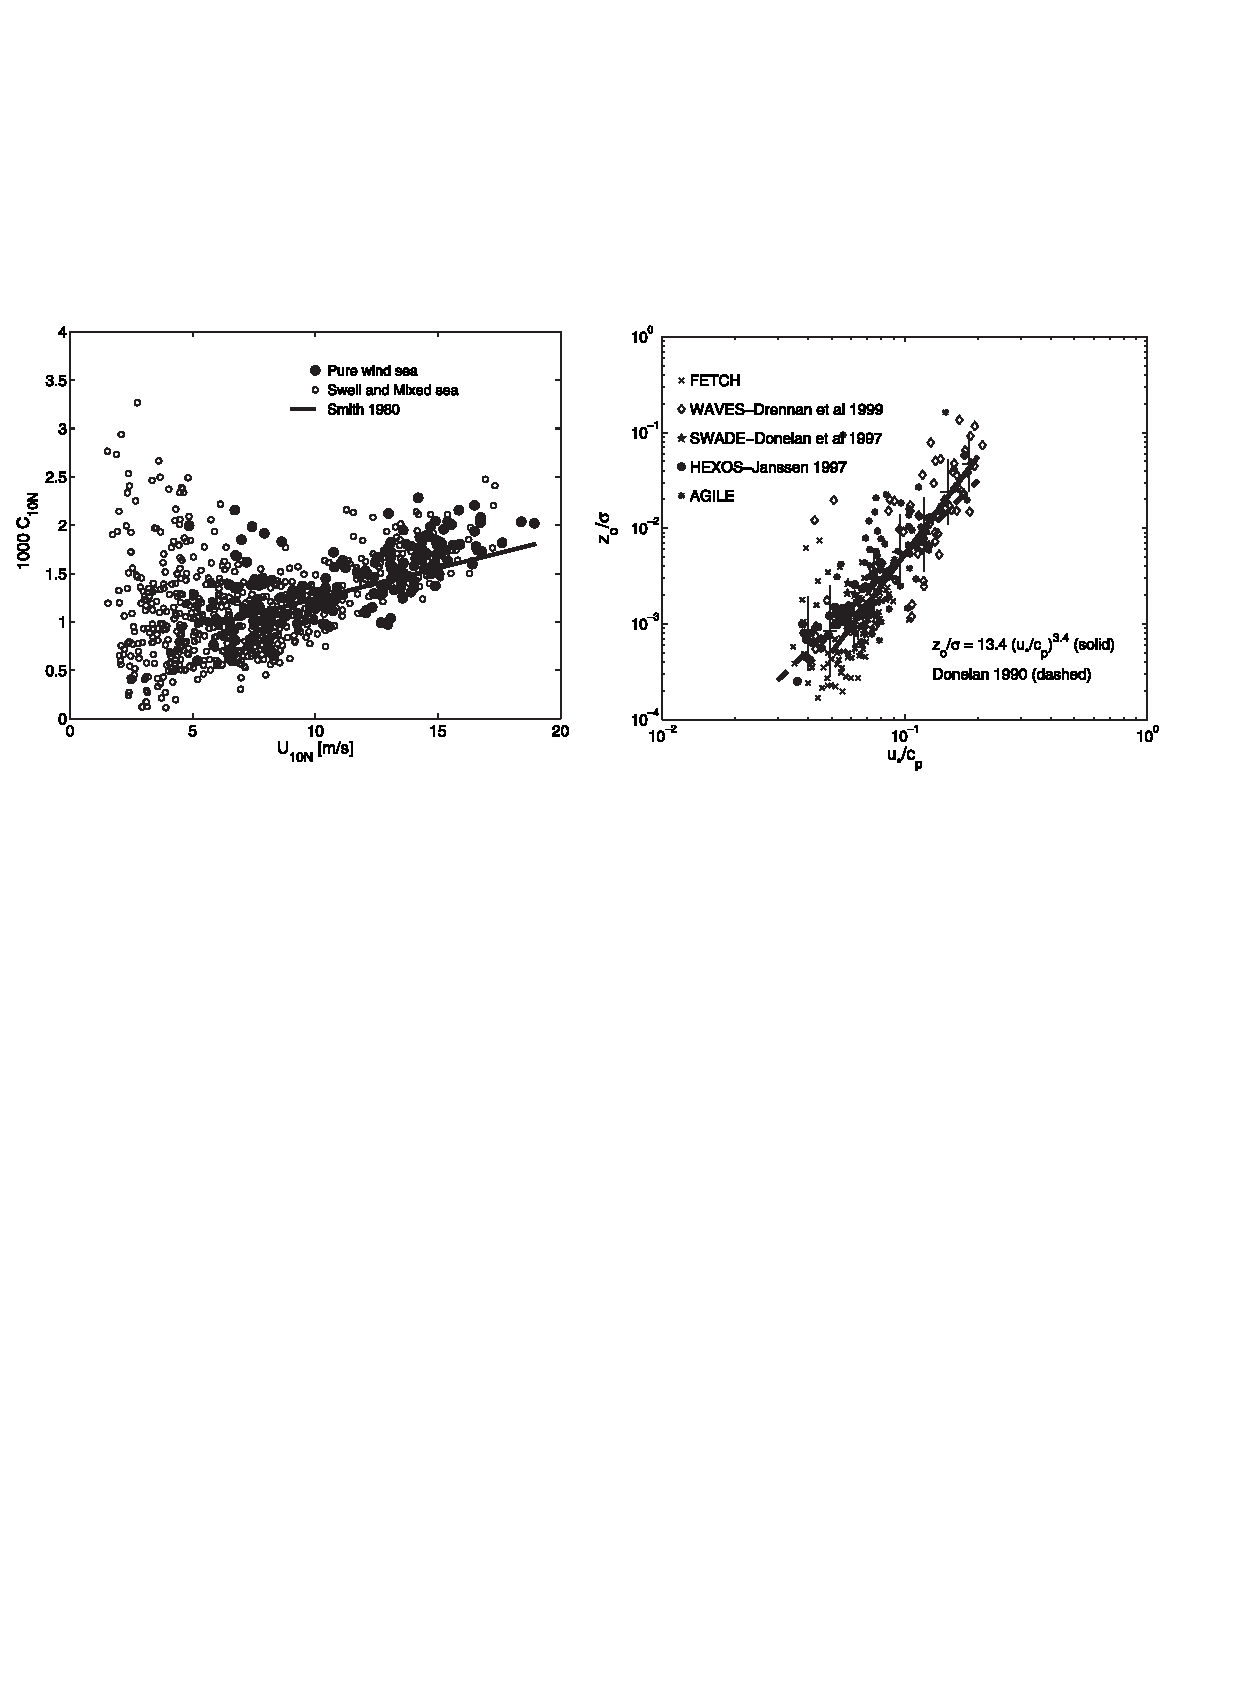
\includegraphics[width=\textwidth]{FIGS_CH_AIRSEA/Drennan_etal_JGR2003.pdf}}
%\vspace{3.64in}
  \caption{Effect of sea state on the wind stress.}{Left: measured neutral drag coefficient  $C_{10N}$, 
  during the  FETCH experiment in the Mediterranean. Right: variation of the roughness length  $z_0$, normalized by a typical wave amplitude $\sigma=H_s/2$ for various experiments. Figure reproduced from \cite{Drennan&al.2003}.}
\label{Drennanetal2003}
\end{figure}
%%%%%%%%%%%%%%%%%%%%%%%%%%%%

However, in general the wave age is correlated to the wind speed, so that it is very difficult to isolate wave age effects. In their recent review of wind stress parameterization for wind speeds 0 to 25 m/s, \cite{Edson&al.2013} concluded that the updated COARE 3.5 parameterization gives a good reproduction of the wind stress as a function of the neutral wind speed alone. 

For higher wind speeds, several estimates of the stress suggest that the value of $C_d$ may decrease, possibly associated to a full separation of the boundary layer. Figure \ref{Lucia2017} shows several drag coefficient from observations and as used in the ECMWF atmospheric model, for which the drag takes into account the waves \citep{Janssen2004}. %Interestingly the ECMWF drag is relatively high and the ECMWF winds are relatively low compared to measurement from platforms. 
%%%%%%%%%%%%%%%%%%%%%%%%%%%%%%%
\begin{figure}[h]
\centerline{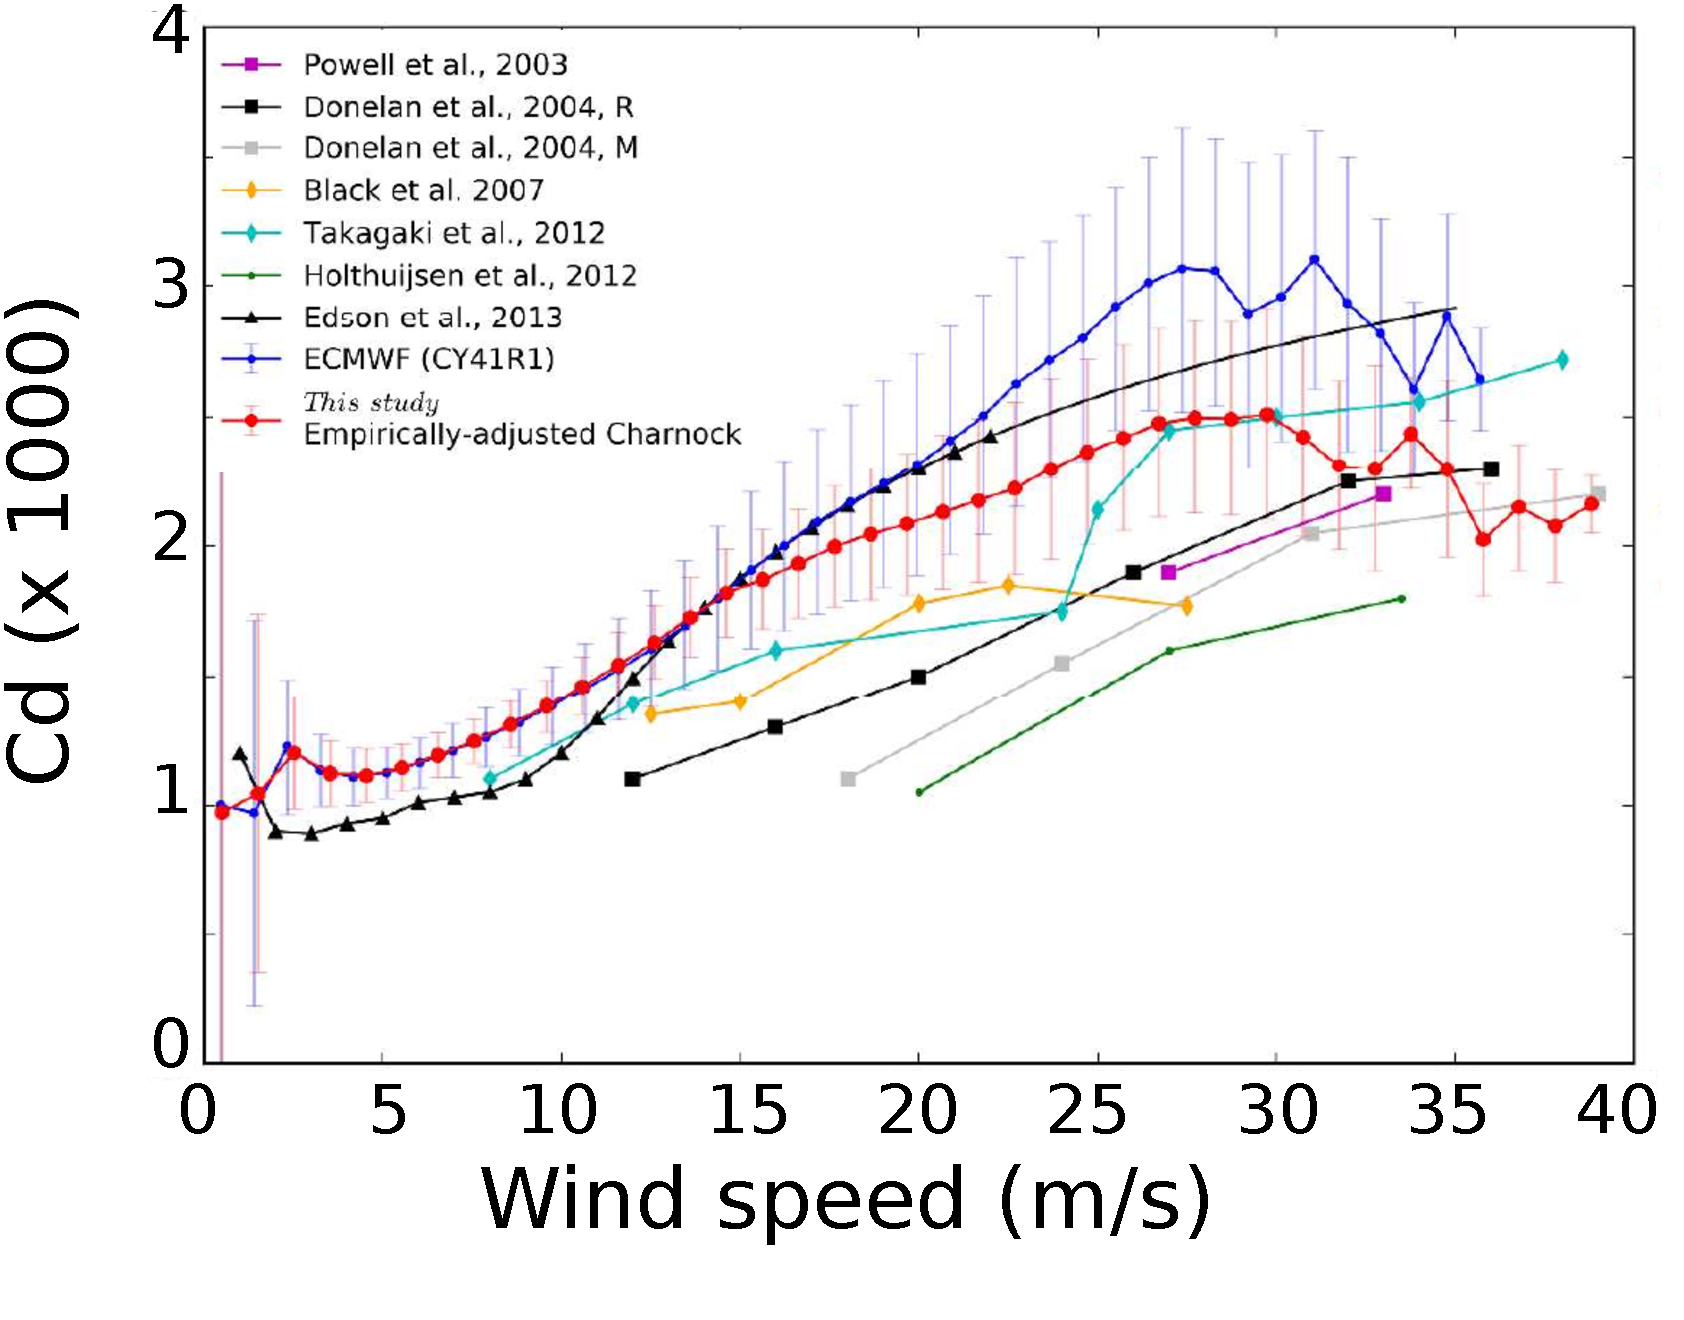
\includegraphics[width=0.6\textwidth]{FIGS_CH_AIRSEA/High_drag_coeff.pdf}}
%\vspace{3.64in}
  \caption{Left: Comparison of drag coefficient for ECMWF (CY41R1) parameterization, empirically-adjusted Charnock parameterization and observations (Donelan et al., 2004, 'R' or 'M' corresponds to different measurements techniques Reynolds or Momentum Budget. %Right: Wind speed biases, on the period 23 to 27 of January 2014 on North East Atlantic, between (a) ASCAT-KNMI, (b) ASCAT-RSS, (c)AMSR2, (d) WindSat, (e) buoys, (f) platforms and model for the default ECMWF CY41R1 (blue) and empirically-adjusted (red) parameterizations.  
%  Beyond 30~m/s, values are plotted as points, representing the large uncertainties on observations.  
  Adapted from \cite{Pineau-Guillou&al.2018}.}
\label{Lucia2017}
\end{figure}
%%%%%%%%%%%%%%%%%%%%%%%%%%%%
%We also note that wind speeds derived from satellite radiometers and scatterometers are not direct measurements and thus depend on the choice and tuning of a Geophysical Model Function that translates the measured quantity (brightness temperature or backscatter) into wind speed. For example the winds from the ASCAT scatterometer processed by KNMI and RSS differ by 7 m/s on average for 30 m/s winds. 

\subsection{Swell and stress direction}
Besides the magnitude of the wind stress, waves also modify the stress direction. This is particularly noticeable at low wind speeds in the presence of swell. Indeed, the wind stress may be opposite to the wind direction for wind speeds below 3 m/s, as the wave are loosing momentum to the atmosphere and generating a low-level jet of wave-driven wind \citep{Semedo&al.2009,Hogstrom&al.2009}. It is more frequent to observe systematic deviations of the wind stress and wind speed directions when waves and wind are not aligned \citep{Potter&al.2015}. 

\subsection{Other effects}
Waves generally have an impact on all air-sea exchanges, not just momentum. This includes mass fluxe \citep[see][ for a recent review of spray generation]{Veron2015} and gas transfer \citep[e.g.][]{Brumer&al.2017b}. Also in the presence of an ice layer, wave-ice interactions should be taken into account. These are discussed in chapter \ref{ch_ice}. 

\section{Drift and mixing}
\subsection{Momentum flux for the Eulerian mean current}
Knowing the wind stress is a first step in determining how the ocean is forced, but this is not enough to tell how much of that momentum goes into currents as most of it generally goes through the wave field. It is only when the wave momentum is constant that the momentum flux from the wind goes entirely to the ocean circulation. In general, we can use the wave energy balance with source terms $S_{\rm in}$ and $S_{\rm dis}$ presented in Chapter \ref{ch_sourceterms}, to compute the wave momentum balance. This was done at the end of Chapter \ref{ch_current}, when we introduced the momentum flux from wind to waves $\tau^{\mathrm{aw}}$ and the flux from waves to ocean $\tau^{\mathrm{wo}}$ .

\subsection{Quasi-Eulerian currents}
The interaction of waves and currents is the topic of onging research, in particular the effects of vertically sheared currents on the waves. 
A general description of these interaction in three dimensions is given in Part 3. Here 
we will consider the much more simple case of a horizontally homogeneous ocean. The wave-averaged momentum equation for the mean current $ \widehat{\mathbf u}$
then takes the following form \citep{Hasselmann1970,Xu&Bowen1994}, 
\begin{equation}
 \frac{\partial \widehat{\mathbf u}}{\partial t}
  = 
 - f {\mathbf e}_z \times \left(\widehat{\mathbf u}+{\mathbf U}_{s}\right) + \frac{\partial}{\partial z} \left[{K_z} \frac{\partial
\widehat{\mathbf u} }{\partial z}\right] - {\mathbf T}^{\mathrm{wo}} 
 \label{avgmomz2}
\end{equation}

The solution is determined by the surface boundary conditions, and the profiles of the mixing coefficient $K_z$,  
and the total momentum injected by the waves ${\mathbf T}^{\mathrm{wo}}$ which is a depth-distributed force such that the momentum flux is 
\begin{equation}
\tau^{\mathrm{wo}}_{\alpha} = \int_{-h}^{\overline{\zeta}} T^{\mathrm{wo}}_{\alpha} {\mathrm d}z = \int \frac{\rho_w g}{C}\left[ S_{\mathrm{tot}}(f,\theta) -S_{\mathrm{atm}}(f,\theta)  \right] {\mathrm d}f {\mathrm d} \theta 
 \end{equation}
 with the source terms $S$ defined in Chapter \ref{ch_sourceterms}. 
 
The current can be obtained by solving  (\ref{avgmomz2}) with a turbulent closure that gives an estimate of  $K_z$. 
Following Prandtl (1904), the usual turbulence closure has an addy viscosity that increases with the distance from the boundary 
\citep{Schlichting1979} and involves a velocity scale $q$ associated to the turbulent motion, 
\begin{equation}
K_z = q S_M l,
\end{equation}
where the turbulent kinetic energy per unit mass is  $q^2 = \overline{u^\prime_i u^\prime_i}$, $S_M \simeq 0.39$ is a constant. 
With this, the  most simple model uses a prescribed mixing length $l$ that is the maximum distance from the surface or the base of the mixed layer. 
\begin{eqnarray}
l &= &\max\left\{-\kappa D_m \varsigma, \kappa  z_{0-}\right\} \quad
\textrm{for}
\quad (-h+\overline{\zeta})/2 < z < \overline{\zeta} \nonumber\\
l &= &\max\left\{\kappa D_m (1+\varsigma), \kappa z_{0b}\right\} \quad
\textrm{for} \quad   -h < z  <(-h+\overline{\zeta})/2 ,
\end{eqnarray}
where $D_m$ is the thickness of the mixed layer. The roughness length  $z_{0-}$ yields a non-zero value of  $K_z$ at the surface, 
  which is consistent with measurements \citep[e.g.][]{Kitaigorodskii1994}. \cite{Thorpe&al.2003a} 
  and other authors have suggested that $z_0$ is of the order of  $H_s$, the significant wave height, and should be more precisely related to the height of the breaking waves\footnote{Ocean circulation models before the year 2000 
  used to ignore these effects, and could have very small values of $K_z$ at the surface, e.g. \citet{Large&al.1994}, 
which could give highly unrealistic values of the surface drift when using very high vertical resolutions.}. 

More complex models consider also an equation of evolution for $q$,  and one must also define the surface boundary
condition for $q$. For example  \cite{Mellor&Yamada1982} use the following equations
\begin{eqnarray}
l q S_q \frac{\partial q^2}{\partial z}  =  \alpha_{\mathrm{CB}} \frac{\rho_a^0}{\rho_w^0}
u_\star^3  \quad \textrm{at} \quad \varsigma =
0, \label{surfq} \\
l q S_q \frac{\partial q^2}{\partial z}  =0 \quad \textrm{at} \quad \varsigma =
-1,
\end{eqnarray}
where $S_q=0.2$. The mixing coefficient for $q^2$ is  $l q S_q$, and 
$\alpha_{\mathrm{CB}}$ is the ratio of the energy flux coming from ocean waves (presumably due to wave breaking), and the fruction velocity cubed. 
This coefficient was particulary discussed by \cite{Craig&Banner1994} and many following authors 
\citep{Terray&al.2000,Mellor&Blumberg2004,Rascle&Ardhuin2009,Rascle&Ardhuin2013}. 
Typically $\alpha_{\mathrm{CB}}$ is of the order of  $100$.

For a simple estimation we consider a fully developed sea state, and we assume that   ${\mathbf
T}^{\mathrm{wo}}$ is concentrated near the surface so that  
we can replace these terms in 
(\ref{avgmomz2}) by a local source of momentum in the surface boundary condition. Namely the net momentum flux coming from the wind and waves is balanced by vertical mixing, 
\begin{equation}
{\mathbf \tau}_a - \tau_{\alpha}^{\mathrm{aw}} + \tau_{\alpha}^{\mathrm{wo}}=
 \rho_w K_z \frac{\partial
\widehat{u}_\alpha}{\partial \varsigma} \quad \textrm{on} \quad \varsigma =0.  \label{surfstress3}
\end{equation}
In fact, in the presence of a strong surface mixing the numerical solution is not very sensitive to the forcing in the boundary condition 
or as a body force concentrated near the surface \citep{Rascle&al.2013}. 

Assuming a fully delveloped sea state the momentum flux $\tau_{\alpha}^{\mathrm{aw}} $  that goes to the wave growth is canceled 
by the dissipation terms and we have
\begin{equation}
{\mathbf \tau}_a  = \rho_w u_\star {\mathbf u}_\star = \rho_w K_z
\frac{\partial \widehat{u}_\alpha}{\partial \varsigma} \quad \textrm{on} \quad
\varsigma = 0, \label{surfstress4}
\end{equation}
with $u_\star$ is the wind friction velocity.

%%%%%%%%%%%%% figure
\begin{figure}
\centerline{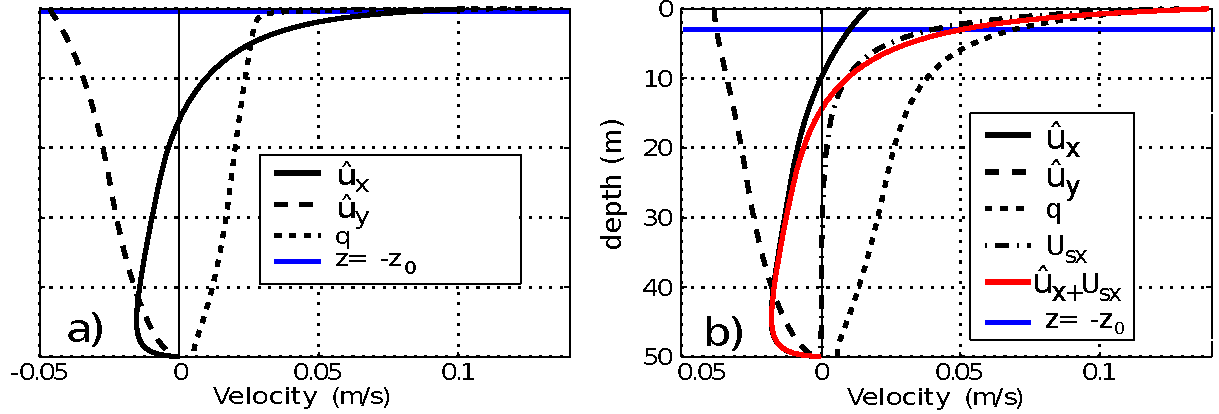
\includegraphics[width=\textwidth]{FIGS_CH_AIRSEA/profil1_en.pdf}}
  \caption{Upper ocean current profiles for a wind speed $U_{10}=10$~m/s}
 {(a) Profiles with a very low value of $z_0$, representing an unrealistic situation without waves 
  (b) profiles with a realistic value of $z_0$. In terms of drift velocity, the much lower value of the surface current is compensated 
  by the Stokes drift.  The velocity scale $q$ is the square root of the turbulent kinetic enenergy (TKE). A realistic surface flux of $q$ is
  needed to get the realistic TKE profile in (b).  (Figure courtesy  of Nicolas Rascle).} \label{fig:2}
\end{figure}
%%%%%%%%%%%%% end of figure

Until the 1990s, all ocean circulation models used very small values of mixing at the surface \citep[e.g.][]{Large&al.1994}, corresponding 
here to low values of $z_{0-}$, such as in Figure \ref{fig:2}.a. This can give very high values of the surface current,s depending on the vertical resolution, 
up to the usally observed 3\% of the wind speed 
\citep{Huang1979} or more. But \cite{Agrawal&al.1992} found that the disspation of TKE was much higher in reality, by at least 
one order of magnitude, so that the mixing must have been strongly underestimated.  Recent models have clearly shown that 
higher surface mixing values are more realistic. For example \cite{Mellor&Blumberg2004} use  $z_0=0.8 H_s$ to get a better fit to measure sea surface temperatures 
in the Gulf of Alaska. This gives a much weaker surface quasi-Eulerian velocity.  This mixing induced by wave breaking is particularly important for 
relatively shallow mixed layers such as found in the Arabian Sea in summer \citep{Janssen2012}, or caused by the diurnal cycle of heating \citep{Noh1996,Noh&Kim1999}.

%%%%%%%%%%%%% figure
\begin{figure}
\centerline{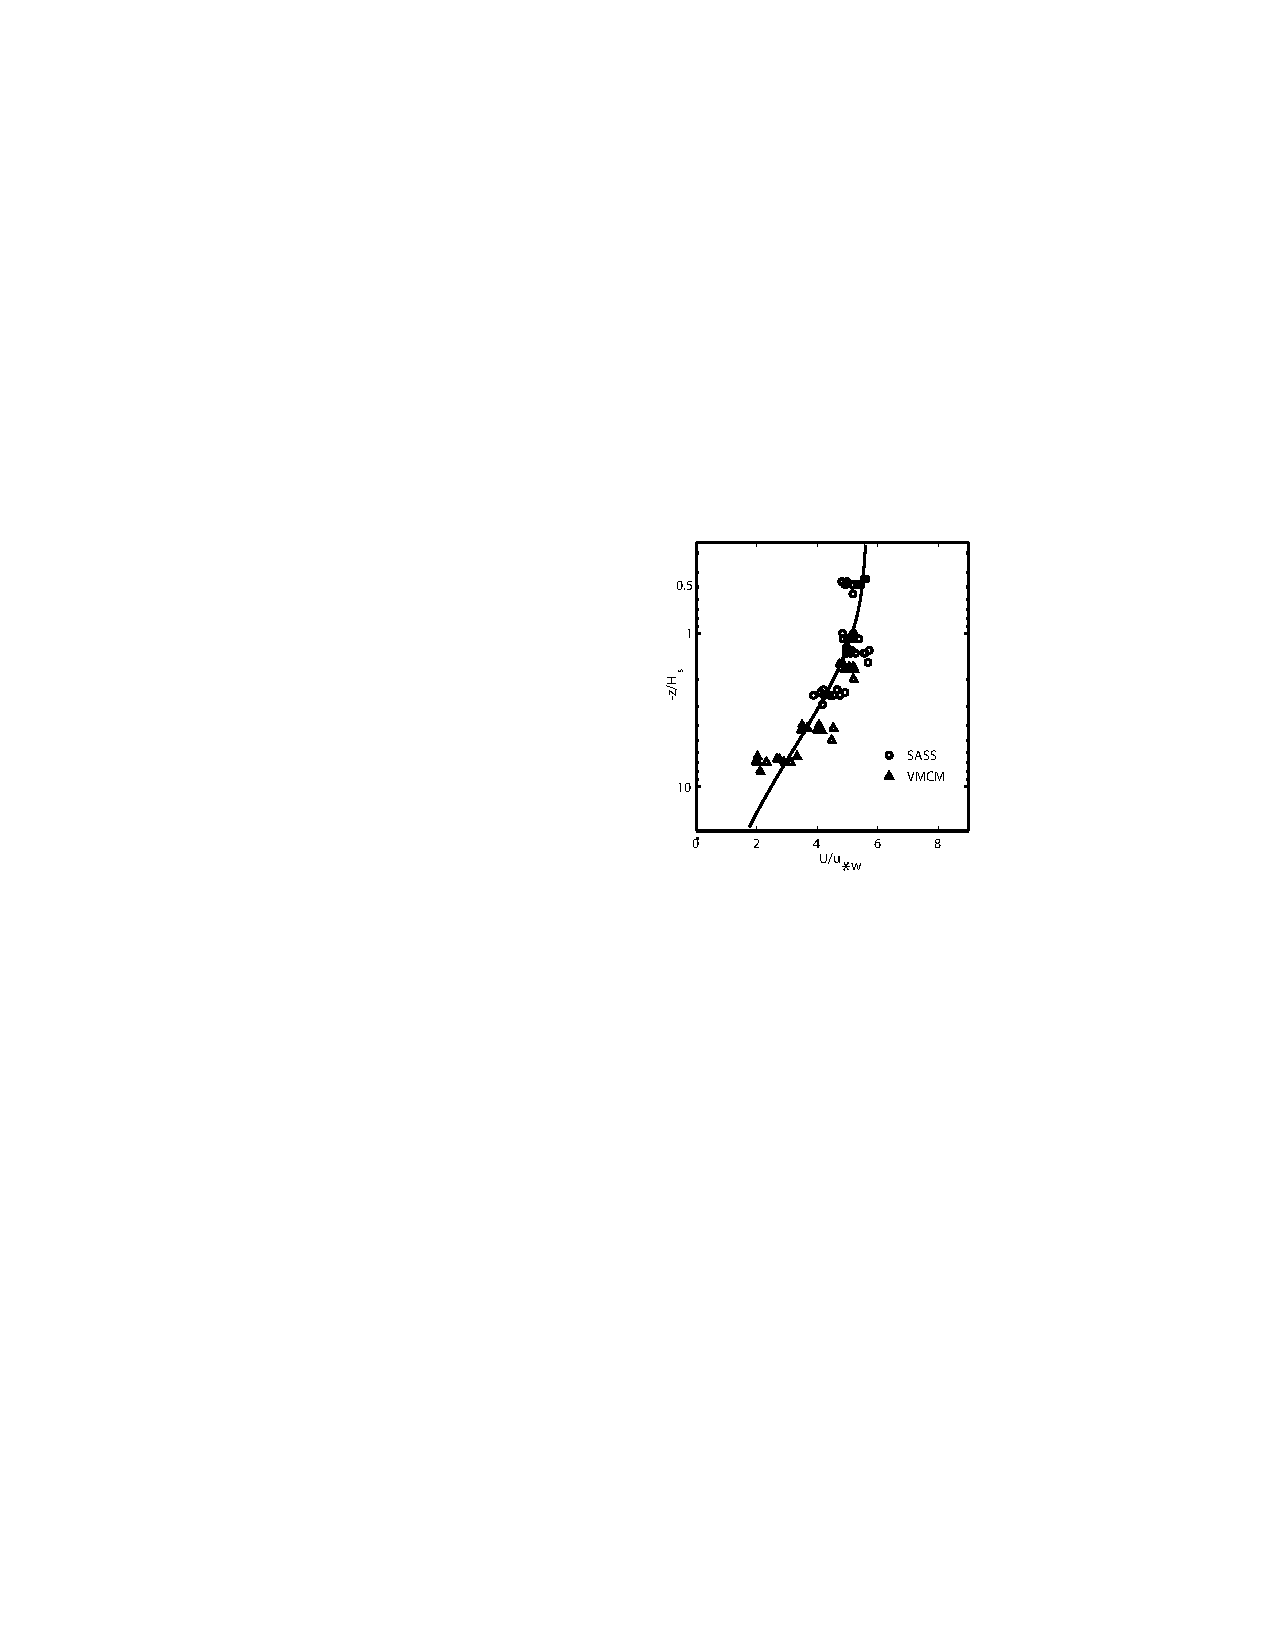
\includegraphics[width=0.4\textwidth]{FIGS_CH_AIRSEA/Terray_etal2000_p5.pdf}}
  \caption{Quasi-Eulerian velocities near the sea surface.}{Two types of current-meters  (SASS and VMCM) provide mean current velocities that have been corrected for wave motion. $u_{\star w}=(\rho_a/\rho_w)^{1/2} u_{\star}$ is the friction velocity in the water (Figure from Terray et al. 2000)\nocite{Terray&al.2000}. The difference in current velocity between the surface and the thermocline is of the order of  0.5\% 
  of the wind speed $U_{10}$.} \label{fig_Santala}
\end{figure}
%%%%%%%%%%%%% end of figure
There are very few measurements of velocity profiles of Eulerian or Lagrangian velocity within the upper 
few meters of the surface. Observations by \cite{Santala&Terray1992} show an Eulerian current that does not exceed  0.5\% of the wind 
speed, see fiugre
\ref{fig_Santala}. 
How general is that? Is it still true if we can measure within a few centimeters of the surface, or right at the surface? 
This is not known yet but several techniques using thermal imagery or polarimetry and wave dispersion should be able to answer these questions. 


\subsection{Stokes drift}
The difference between the Lagragian mean velocity, which is the speed or water particles and the speed that advects tracers (temperature, salinity ...), and the quasi-Eulerian velocity is the Stokes drift. To lowest order, this Stokes drift can be computed from the wave spectrum (Chapter \ref{ch_momentum}). For random wave field in deep water, eq. (\ref{eq:Us_mono_deep}) gives \citep{Kenyon1969},
\begin{eqnarray}
 U_s (z)&=& \int\int 2 \sigma k \cos(\theta) E(f,\theta) \exp(2kz) {\mathrm d}f {\mathrm d} \theta, \\
 V_s (z)&=& \int\int 2 \sigma k \sin(\theta) E(f,\theta) \exp(2kz) {\mathrm d}f {\mathrm d} \theta.
\end{eqnarray}
%%%%%%%%%%%%%%%%%%%%%%%%%%
\begin{figure}[htb]
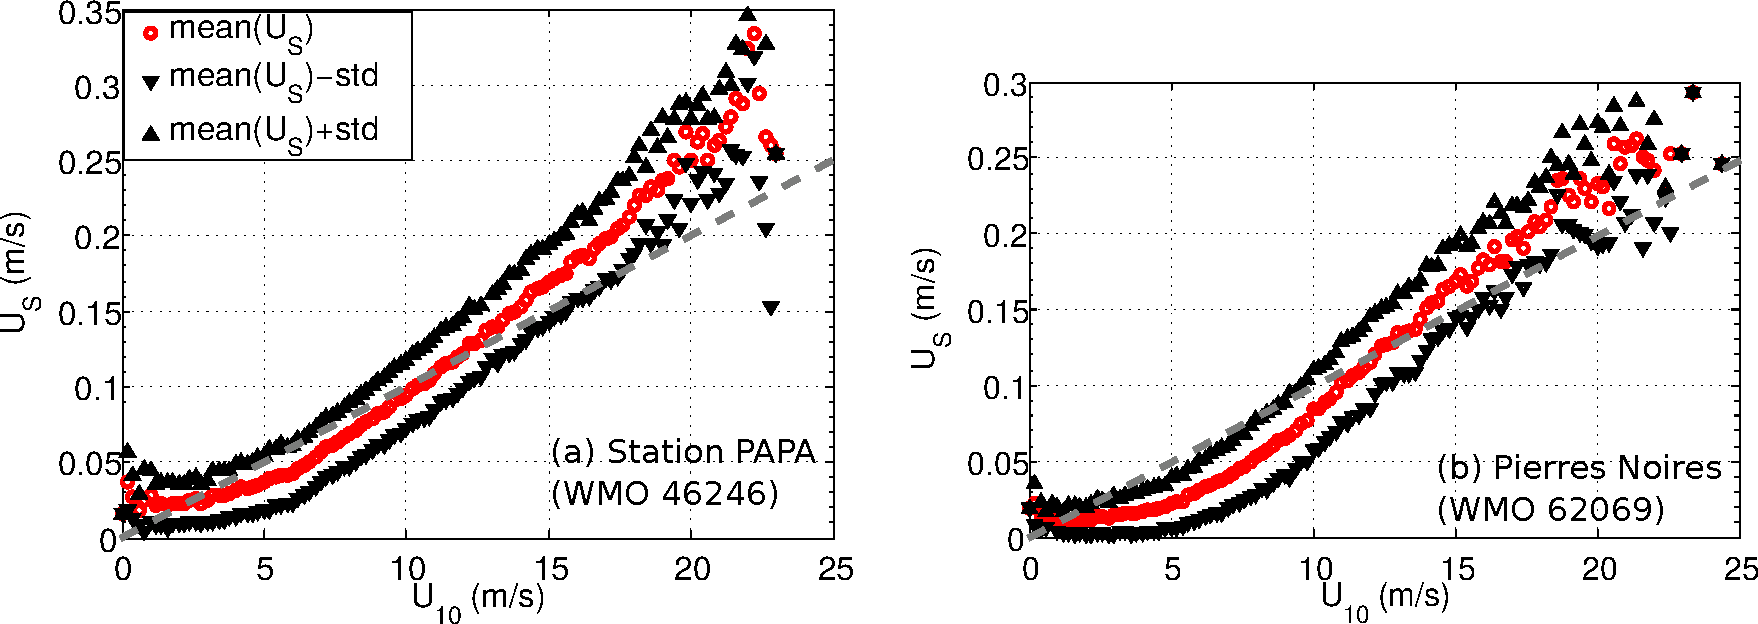
\includegraphics[width=0.9\linewidth]{FIGS_CH_AIRSEA/Us_PAPA_62069_line.pdf}
\caption{Example of mean value (in red) of the surface Stokes drift vector norm $U_{ss}=|(U_{ss},V_{ss})|$ as a function of wind speed for two locations: station PAPA in the North-East Pacific, and buoy 62069 off the French Atlantic coast. These are obtained by integrating the wave spectrum up to 0.5~Hz. The black symbols show the mean plus or minus one standard deviation for each wind speed. The dashed grey line is $U_S = 0.01 U_{10}$.   \label{fig:USU10}}
\end{figure}
%%%%%%%%%%%%%%%%%%%%%%%%%%


Clearly this expression has a strong contribution from short waves, and thus should be largely influenced by the local wind. 
Still, for any given wind speed, the surface Stokes drift value $U_{Ss}$ has a root mean square variability of the order of 40\%, particularly for relatively low wind speeds, below 7~m/s, as shown in figure \ref{fig:USU10}.

Based on direction spectra measured by surface-following buoys, 
\cite{Ardhuin&al.2009} found that the surface Stokes drift  $U_{\mathrm{Ss}}$ could be estimated fairly accurately, with a root-mean-square error of the order of 20\%, by an expression as a function of the wind speed and wave height, 
\begin{equation}
U_{\mathrm{Ss}}(f_c)\simeq 3.7\times 10^{-4}
\left[1.25-0.25\left(\frac{0.5}{f_c}\right)^{1.3}\right] U_{10}
 \min\left\{U_{10},14.5\right\} + 0.025\left(
H_s-0.4\right),\label{Uss_U10}
\end{equation}
in which  $f_c$ is the frequency up to which the Stokes drift is taken into account. This 
expression was validated for $0.3<f_c<0.6$~Hz. 




When subtracting this Stokes drift from HF radar data they found that the quasi-Eulerian current was of the order of 0.4 to 0.8\% of the wind speed, with important variations due to inertial oscillations, and, in the Northern hemisphere, a mean direction 60 degrees to the right of the wind. The model proposed here adds the Stokes drift to the quasi-Eulerian velocity and matches relatively well observations of surface drift and mixing  \citep{Rascle&al.2006}. The effect of stratification is particularly discussed by \cite{Rascle&Ardhuin2009}. 

The present model gives both a strong vertical shear of the drift velocity (mostly due to the Stokes drift) and a strong mixing (caused by wave breaking). 
Still the modeled drift is low by  0.5 to 1.5\% of $U_{10}$ compared to the typical 3\% surface drift. One possible reason is that surface drift objects are trapped in convergence zones where the mean velocity is faster than that of the surrounding water. These convergence zones are associated to Langmuir cells. 

\section{Langmuir circulation}
%%%%%%%%%%%%% figure
\begin{figure}
\centerline{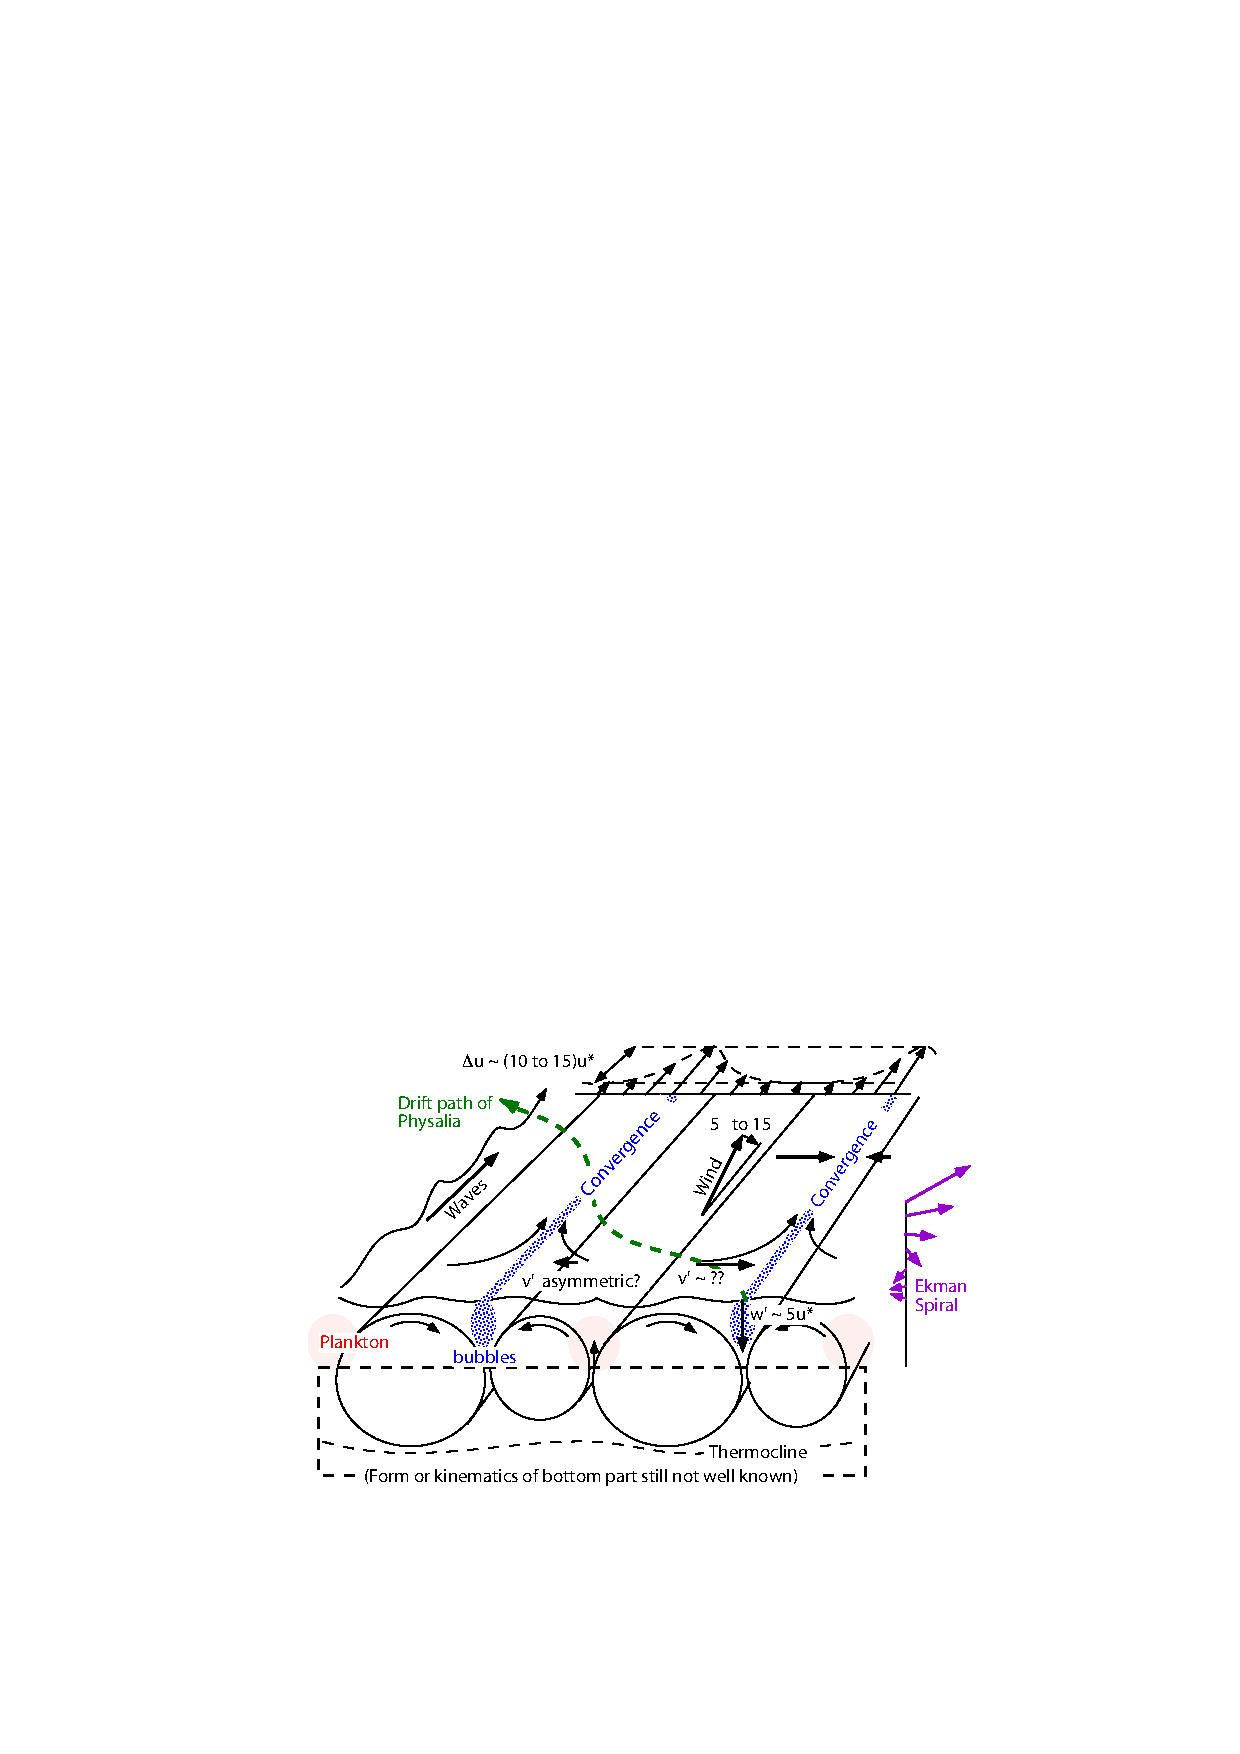
\includegraphics[width=0.7\textwidth]{FIGS_CH_AIRSEA/SmithStoryOfMixing.pdf}}
  \caption{Langmuir cells (figure by J. A. Smith)} \label{fig_Langmuir}
\end{figure}
%%%%%%%%%%%%% end of figure
Indeed the velocities in the upper ocean are not homogeneous horizontally \citep{Weller&al.1985}. Many observations, starting with 
\cite{Langmuir1938} have revealed lines of convergence where foam, flotsam, sargassum and any buoyant material gathers at the surface \citep{Thorpe&al.2003b}. 
These lines are roughly aligned with the wind direction, and correspond to the surface convergence of the rolls that form the Langmuir circulation (Figure \ref{fig_Langmuir}). These rolls emerge due to an instability of the mean vertical shear $\partial \widehat{u}/ \partial z$ that is  stretched by the Stokes 
drift shear $\partial U_s/ \partial z$  and thus get their energy from the wave field via the turbulent kinetic energy production term $\overline{u'w'}\partial U_s/\partial z$, as detailed in Part 3. The momentum balance that gives 
these rolls was further analyzed by \cite{Suzuki&Fox-Kemper2016}. These rolls have been observed in most experiments in the ocean and in the laboratory \citep[e.g.][]{Thorpe1992,Melville&al.1998,Smith1999}, including in shallow water \citep{Marmorino&al.2005}. They are well reproduced in Large Eddy Simulations \citep[e.g.][]{Noh&al.2004,Harcourt&DAsaro2006,Sullivan&McWilliams2010} and can interact with mixed layer fronts \citep{Suzuki&al.2016}.

The parameterization of Langmuir circulation in models that do not resolve them is the topic of active research \citep[e.g.][]{Li&Fox-Kemper2017}. 



\cleardoublepage
\chapter{Waves and ocean remote sensing}\label{ch_tele}
\input{ch_tele}
\cleardoublepage


\part{Waves in coastal and nearshore environments}
\chapter{Linear shoaling, refraction and reflection}\label{ch5}
\input{ch12_en}
\cleardoublepage
\chapter{Nonlinear wave shoaling}\label{ch_surf}
\input{ch_surf_en}
\cleardoublepage
\chapter{Bottom boundary layer: processes and parameterizations}\label{ch_wbbl}
\input{ch_wbbl_en}
\cleardoublepage
\chapter{Wave-driven nearshore flows: water levels and currents}\label{ch_littoral}
\input{ch_nearshore_en}
\cleardoublepage
\chapter{Numerical wave modelling at regional to beach scales}\label{ch_model_coastal}
\input{ch_model_coastal_en}
\cleardoublepage


\appendix
\chapter{Some useful tables}
 %%%%%%%%%%%%%%%%%%%%%%%%%%%%%%%%%%%%%%%%%%
\begin{table}
  \centering
  \begin{tabular}{cccccc}
\hline
    $Y=X\tanh(X)$ & $X$     & $Y=X\tanh(X)$ & $X$   & $Y=X\tanh(X)$ & $X$\\
 \hline
       0.05    &     0.2255   &     1.30 & 1.4511 &     2.55  &      2.5795   \\
       0.10    &     0.3216   &     1.35 & 1.4934 &     2.60  &      2.6273   \\
       0.15    &     0.3973   &     1.40 & 1.5360 &     2.65  &      2.6753   \\
       0.20    &     0.4627   &     1.45 & 1.5788 &     2.70  &      2.7234   \\
       0.25    &     0.5218   &     1.50 & 1.6218 &     2.75  &      2.7716   \\
       0.30    &     0.5767   &     1.55 & 1.6651 &     2.80  &      2.8200   \\
       0.35    &     0.6284   &     1.60 & 1.7085 &     2.85  &      2.8684   \\
       0.40    &     0.6778   &     1.65 & 1.7523 &     2.90  &      2.9170   \\
       0.45    &     0.7255   &     1.70 & 1.7962 &     2.95  &      2.9657   \\
       0.50    &     0.7717   &     1.75 & 1.8405 &     3.00  &      3.0145   \\
       0.55    &     0.8168   &     1.80 & 1.8850 &     3.05  &      3.0634   \\
       0.60    &     0.8611   &     1.85 & 1.9297 &     3.10  &      3.1123   \\
       0.65    &     0.9046   &     1.90 & 1.9747 &     3.15  &      3.1613   \\
       0.70    &     0.9476   &     1.95 & 2.0199 &     3.20  &      3.2104   \\
       0.75    &     0.9902   &     2.00 & 2.0653 &     3.25  &      3.2596   \\
       0.80    &     1.0324   &     2.05 & 2.1110 &     3.30  &      3.3088   \\
       0.85    &     1.0744   &     2.10 & 2.1570 &     3.35  &      3.3581   \\
       0.90    &     1.1163   &     2.15 & 2.2031 &     3.40  &      3.4075   \\
       0.95    &     1.1580   &     2.20 & 2.2495 &     3.45  &      3.4569   \\
       1.00    &     1.1997   &     2.25 & 2.2961 &     3.50  &      3.5063   \\
       1.05    &     1.2414   &     2.30 & 2.3428 &   &     \\
       1.10    &     1.2831   &     2.35 & 2.3898 &   &     \\
       1.15    &     1.3249   &     2.40 & 2.4370 &   &     \\
       1.20    &     1.3668   &     2.45 & 2.4843 &   &     \\
       1.25    &     1.4088   &     2.50 & 2.5318 &   &     \\
    \hline                  
\hline
\end{tabular}
  \caption{Table of the inverse function of $X \tanh X$. Defining $Y=\sigma^2 D/g$ it gives $k=X/D$, 
which allows to invert the dispersion relation in the absence of current. 
For $Y< 0.05$ one should use $X=\sqrt{Y}$, and for $Y >3.5$ one should use $X=Y$.}\label{table_tracks}
\end{table}
%%%%%%%%%%%%%%%%%%%%%%%%%%%%%%%%%%%%

%%%%%%%%%%%%%%%%%%%%%%%%%%%%%%%%%%%%%%%%%%%%%%%%%%%%%%%%%%%%%%%%%%%%%%%%%%%%
\begin{figure}
\centerline{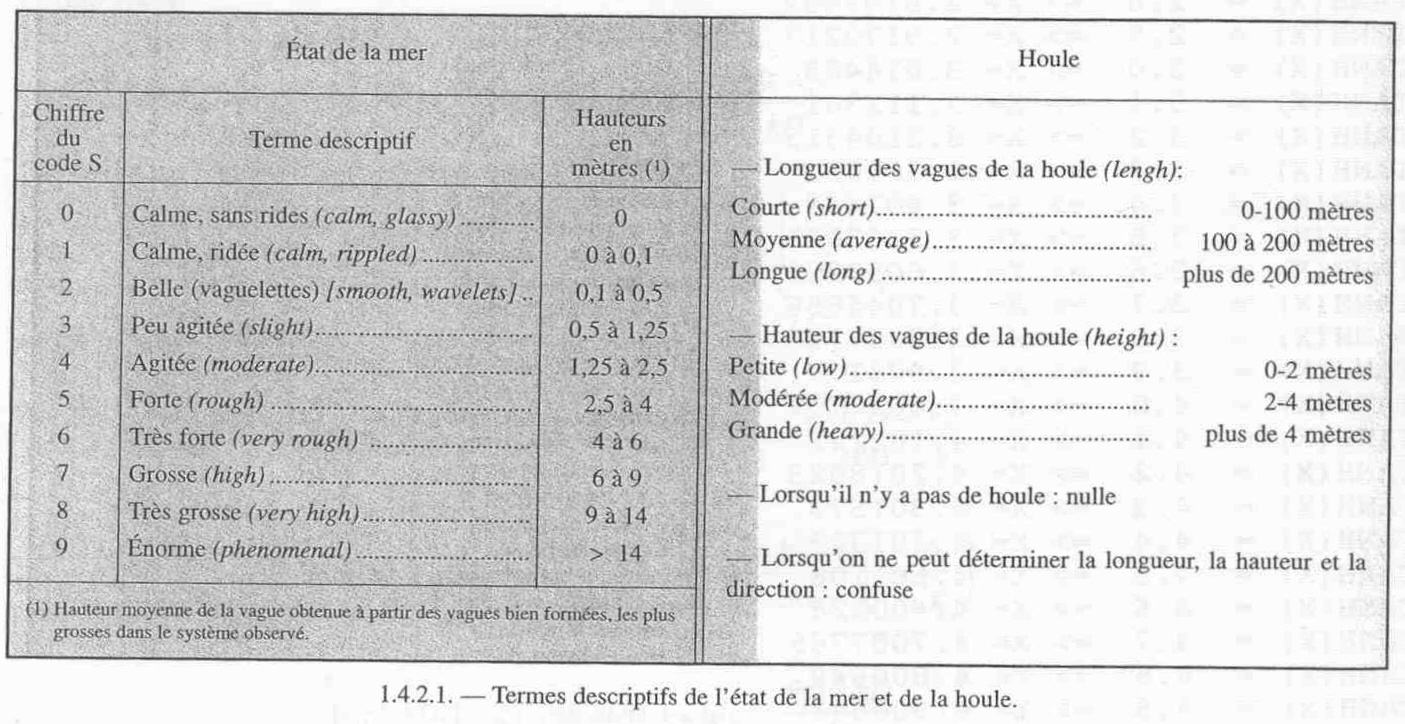
\includegraphics[width=\textwidth]{FIGURES/Table_Beaufort.jpg}}
%\vspace{3.64in}
\caption{The Beaufort scale for sea states \label{table_beaufort}}
\end{figure}
%%%%%%%%%%%%%%%%%%%%%%%%%%%%%%%%%%%%%%%%%%%%%%%%%%%%%%%%%%%%%%%%%%%%%%%%%%%%


%\bibliographystyle{ametsocjmk_nourl}   % si on n'utilise pas  hyperref
\bibliographystyle{ametsocjmk_en}         % avec  hyperref
\bibliography{wave}  % see main.bib; used BibTeX to generate main.bbl




\end{document}        % That's All, Folks!
